%\documentstyle[graphicx,natbib]{article}
\documentclass[11pt]{article}
\usepackage{aas_macros}
\usepackage{graphicx}
\usepackage[numbers]{natbib}
\usepackage{hyperref}


\setlength{\parskip}{2ex}
\setlength{\parindent}{2em}
\setlength{\textwidth}{16cm}
\setlength{\textheight}{23cm}
\setlength{\oddsidemargin}{0.25cm}
\setlength{\evensidemargin}{0.25cm}
%\setlength{\topmargin}{-2.0cm}         % Zurich
\setlength{\topmargin}{-1.5cm}         % Bern
\def\thefootnote{\fnsymbol{footnote}}

\setlength{\parindent}{0pt} % No indent

\renewcommand{\thesection}{\Alph{section}}
\renewcommand{\thesubsection}{\arabic{subsection}}


%\def\mnras{\ref@jnl{MNRAS}}


%-----------------------------------------------------------------------

\begin{document}

\newpage

\section*{Research Plan}

\begin{abstract}
Blabla
\end{abstract}


\subsection{Introduction and Status of Research}
\label{sec:intro}

\subsubsection{General relativity and gravitational lenses}

In the year 1915, Albert Einstein published the theory of General Relativity (GR).
This theory describes the interplay of matter (energy and impulse) and space-time and the perturbations on the latter caused by the former.
GR allowed the first time to correctly describe the anomalous precession of Mercury.
The next experimental proof of GR was the deflection of the light of a star by the sun (by Eddington in the year 1919).
Einstein already predicted this phenomena in 1911 up to a factor of two.
This was the starting shoot for Einstein’s second great theory and first observation and evidence of \emph{(micro) gravitational lensing}\footnote{Even thou the accuracy of this measurement was questioned in recent years, see \cite{kennefick2009testing}}.

Gravitational Lensing (GL) describes the phenomena of deflection of light around a massive object, due to the deflections in space-time caused by the mass.
Quite similar to the deflection of the path of a marble rolling on a rubber sheet, stretched by a mass in it's centre.
If the source of the light (``source''), the massive object (``lens'') and the observer align approximately in a line, these distortions act similar to a regular lens.
Depending on the configuration, a background light source is distorted, magnified or even multiplied, as shown in Fig.~\ref{fig:grav_lens}.

\begin{figure}[h]
	\centering
		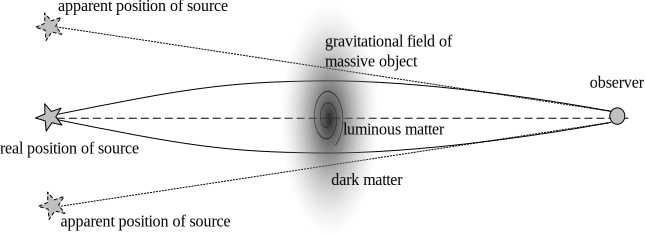
\includegraphics[width=0.75\textwidth]{img/grav_lens}
	\caption{Schematics of gravitational lensing}
	\label{fig:grav_lens}
\end{figure}

This phenomena is divided into three sub categories:
\begin{itemize}
	\item \emph{Strong lensing} occurs if the lens is extremely massive. Consider a single galaxy, galaxy clusters or black holes.
Strong lensing allows not only for displacements of sources, but for magnification and creation of multiple images.
The first observed strong lensing was the twin quasar Q0957+561 discovered 1979 (\cite{walsh19790957}).
  \item In contrast, \emph{Weak lensing} phenomena are not directly observable.
The GL caused by a weak or far away gravitational field causes only a distortion of the shape of sources (shear), that can be statistically analysed.
  \item \emph{Micro lensing} deals with tiny perturbations of the perceived light magnitude from a source, caused by gravitational field in the order of single lensing stars.
Micro lensing is used to detect MACHOs\footnote{Massive Astrophysical Compact Halo Object} and extra solar planets.
\end{itemize}

In my work, I'm focussing on strong lensing, since it's directly detectable in astronomical pictures taken by telescopes.


\subsubsection{Finding gravitational lenses}



\subsubsection{Gravitational lens modelling}

Since the effect of gravitational lensing depends on a variety of parameters, the study of gravitational lenses allow an alternative approach of estimating many of those parameters.
The study of a discovered gravitational lens usually involves in a first step to create an accurate model for the source light profile / distribution, the lensing mass distribution and the distances between source, lens and observer.
This process is commonly referred to as ``modelling'' a gravitational lens.
These models allow to tackle down a lot of open questions in current astrophysics and even some general physical questions.

The model of the lensing allows in a first step to estimate total masses of distant (lensing) galaxies.
It takes into account the whole mass of the lens, the visible matter and the dark matter \cite{kochanek1995there}.
Thus it offers an alternative\footnote{Alternative to the approach of particle physics and particle collides like LHC.} approach to tackle down the mystery of dark matter.
It allows the measure the ratio of visible matter to dark matter and the radial distribution of dark matter in galaxies \cite{treukoop04}.
Additionally it allows to test other standard procedures to estimate distant masses \cite{kochanek1995there}.

Models of sources in a gravitational lensing model provides information about potentially very early objects in the universe.
Those object can only be observed, due to the magnification effect of GL and could lead to new information about the early evolution of the universe (\cite{rusin03}).

If two or more images can be observed, there is usually a time delay between those images, since one light path is longer.
This information can be used to narrow down fundamental cosmological parameters, as described in \cite{refsdal1964}.


\subsection{Own Recent and Ongoing Work}

\subsubsection{Motivation}

\subsubsection{My approach}

\subsubsection{MSc thesis: Spaghetti Lens}

\subsubsection{Future work}




\subsection{Resources and Timing}

\subsubsection{Short term: until Sept. 2014}
The prototype of SL is working already, but it needs a few bug fixes and upgrades.
An increase in the modelling resolution in the centre is easy to implement and could improve the approx. 20\% overshoot detected in my Masters thesis.
The hardware upgrade to the new server software would greatly increase usability and stability of the application.
I plan to have this points done by this September 2014 and officially release the first non beta version of SL.

\begin{itemize}
	\item Labs web page online
  \item fix currently known bugs
  \item implement source modelling
  \item increase central resolution
  \item set up the new server
\end{itemize}


\subsubsection{Mid term: Summer 2015}

The first year will be spent, besides the tasks mentioned in section~\ref{sec:ongoing}, in implementing additional modelling features to SL.
As this will be in close collaboration with requests from researcher and volunteers, additional minor point for data analysis and retrieval capabilities will show up.
Currently, the two major upgrades listed below are planned. I aim at having a stable prototype of those by Summer 2015.

Additionally, I will use SL to model all currently known gravitational lenses.
This allows me to produce scientific data to work on in the second year and being independent of the amount of work done by volunteers.


\begin{itemize}
  \item modelling multiple lenses / group lenses (for researchers / professionals)
  \item implement photometry (for volunteers)
\end{itemize}


\subsubsection{Long term: Summer 2016}

For the second year, the prototypes developed in the first year should be deployed.
Besides the work to keep SL running, I intent to use this time to evaluate the generated data and produce publish first analyses and scientific results using alredy generated data.

\begin{itemize}
  \item deploy prototypes
  \item analyse and publish first bits of data generated
\end{itemize}


\subsubsection{Ongoing}
\label{sec:ongoing}

Besides the ongoing development and bug fixing of SL, there are several tasks that will span the whole time of my thesis:
\begin{itemize}
  \item Training and assistance of volunteers: My master thesis has shown, that there is a great demand in assistance and discussing results from the volunteers.
  \item Model all known lenses: Keep up to date with newly discovered lenses and try to have all modelled as soon as discovered.
  \item Publicity: Make the SL project more known, try get new volunteers by going to conferences, offering projects with high school classes, and so on.
\end{itemize}


\subsubsection{Resources}

As mentioned in previous sections, SL currently runs on a mix of outdated hardware and office computers.
Thus it doesn't offer the reliability and speed required for the acceptance and success of such a project amount volunteers and researchers alike.
A one time investment in a decent application server is favourable, and thus I'm requesting additional founds for an application server.

I consider the personal contact to researcher and volunteers as a key component in motivating new volunteers to joint the project.
Thus I'm requesting a yearly budget to travel to conferences and meetings, and to organise projects for schools and other groups to increase the publicity of the project.



\subsection{Scientific Relevance of Expected Results}

The main problems addressed with my thesis is to establish a network of software, volunteers and researchers to provide the scientific community a fast and reliable way to evaluate large amount of gravitational lenses.
When the NASA mission Wide Field Infrared Survey Telescope (WFIRST, to be launched in 2024) and the ESA space telescope Euclid (launch in 2020), the facilities to analyse and model GL in large scale will be required.
We have the opportunity, to build up knowledge and infrastructure to make sure, the data generated by those missions are properly analysed.

%Gravitational lenses detected today usually get modelled by the discoverer.
%Those models are usually published  in the discovery paper.
%We would provide a check using a standartised procedure for all those models.


As a side effect, all kinds of parameters and constants of the universe (as explained in section~\ref{sec:intro}) will be determined or tested directly by my thesis.



\bibliographystyle{bib/rplan}
\bibliography{bib/rplan}


\end{document}

